\documentclass[conference]{IEEEtran}
\IEEEoverridecommandlockouts
\usepackage[backend=biber, sorting=none]{biblatex}\bibliography{references}
\usepackage[hidelinks]{hyperref}
\usepackage{amsmath,amssymb,amsfonts}
\usepackage{algorithmic}
\usepackage{graphicx}
\usepackage{textcomp}
\usepackage{xcolor}
\usepackage{parskip}
\usepackage{tikz}
\usepackage{float}
\usepackage{pgfplots}
\usepgfplotslibrary{colorbrewer}
\usepackage[acronym]{glossaries}
% This is where I define commands and acryonyms; that sort of thing.
\newacronym[plural=SLAs]{SLA}{SLA}{Service Level Agreement}
\newacronym{ILP}{ILP}{Integer Linear Programming}

\renewcommand{\O}[1]{$\mathcal{O}(#1)$}
% Misc config file to do things like use DOIs instead of URLs when both are available.
\DeclareSourcemap{
  \maps[datatype=bibtex]{
    \map[overwrite]{
      \step[fieldsource=doi, final]
      \step[fieldset=url, null]
      \step[fieldset=eprint, null]
    }
  }
}
\graphicspath{ {./images/} }


\begin{document}

\title{The Title of this Paper}

\author{\IEEEauthorblockN{Christopher McMorran}
\IEEEauthorblockA{\textit{Whatever department I'm using this in} \\
\textit{Institution name}\\
myemail@officialsite.extension}}

\maketitle

\begin{abstract}
This is where we can put the abstract.
\end{abstract}

    \section{Introduction}
    \subsection{A subsection after the intro}
    Some text could go here. We can draw fancy graphs with tikz and wrap them in figures like this:
    \begin{figure}[h]
        \centering
            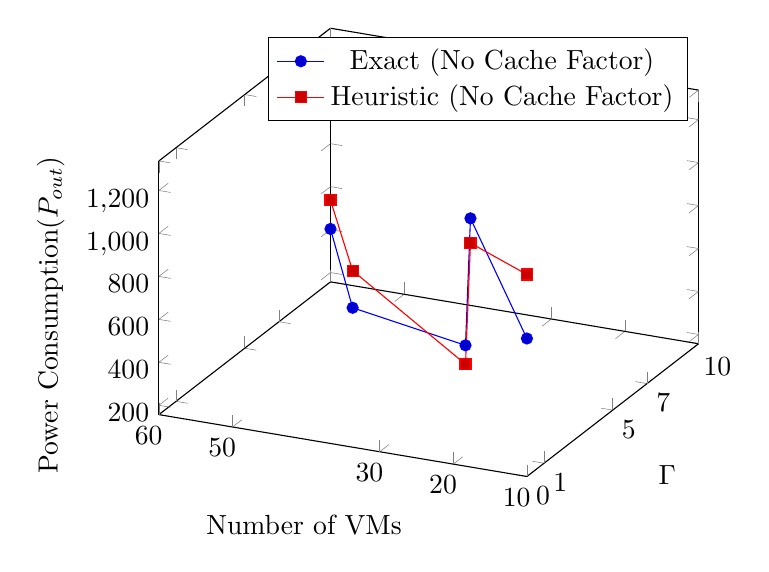
\begin{tikzpicture}
            \begin{axis}[
            xlabel=$\text{Number of VMs}$,xtick=data, x dir=reverse,
            ylabel=$\Gamma$, ytick=data,
                zlabel=$\text{Power Consumption} (P_{out})$, ztick={200, 400, ..., 1400},
            ]
            \addplot3 coordinates {(60, 10, 403) (50, 7, 279) (30, 5, 343) (20, 1, 1239) (10, 0, 799)};
            \addlegendentry{Exact (No Cache Factor)}
            \addplot3 coordinates {(60, 10, 536) (50, 7, 452) (30, 5, 255) (20, 1, 1124) (10, 0, 1097)};
            \addlegendentry{Heuristic (No Cache Factor)}
            \end{axis}
            \end{tikzpicture}
        \caption{Results from a re-implementation of the method proposed by \citeauthor{nasim2017robust}.}
        \label{fig:replication}
    \end{figure}
    We can cite this figure using Figure~\ref{fig:replication}. We can also import images using
    \begin{figure}[h]
        \includegraphics[scale=0.6]{myimg}
        \label{fig:cat}
        \caption{A cat.}
    \end{figure}
    \subsubsection{A sub-subsection}
    Some text could go here. Or maybe a list:
    \begin{enumerate}
        \item {An item}
        \item {Another item}
    \end{enumerate}
    \section{Body}
    We can do centered math like this:
    \[f(c_{j}) = \prod_{k = 1}^{K}C_{k, j}\] 
    \subsubsection{Another sub-subsection}
    Here we would write things about stuff and maybe cite a paper with~\cite{Amdahl:1967:VSP:1465482.1465560}.
    \section{Conclusion}
    Conclude all the things.
    % Generate the list of references based on what we cited.
    \printbibliography
\end{document}